\documentclass[tikz,border=3pt]{standalone}
\usepackage{amsmath,amssymb}
\usetikzlibrary{arrows.meta,positioning,calc,fit,backgrounds}

\definecolor{ink}{HTML}{243447}
\definecolor{blue}{HTML}{4477AA}
\definecolor{cyan}{HTML}{66CCEE}
\definecolor{green}{HTML}{228833}
\definecolor{gold}{HTML}{CCBB44}
\definecolor{rose}{HTML}{CC6677}
\definecolor{papergray}{HTML}{F5F6F7}

\begin{document}
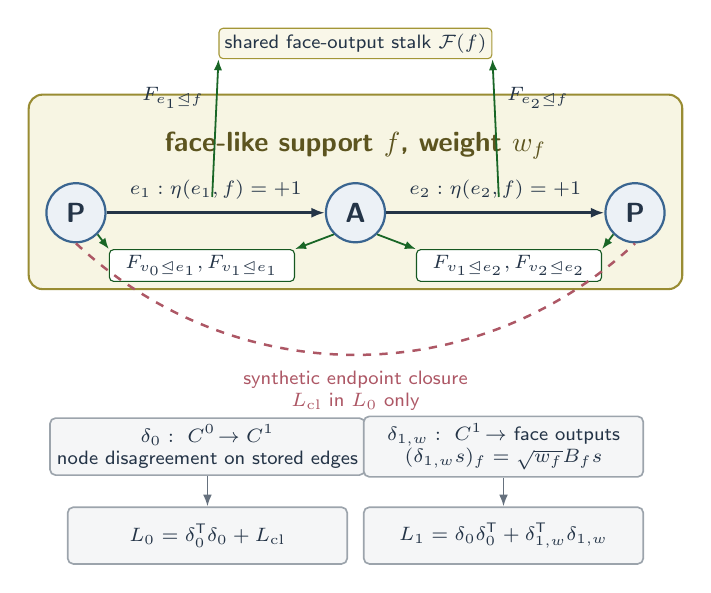
\begin{tikzpicture}[
  font=\sffamily\scriptsize,
  text=ink,
  >=Latex,
  vertex/.style={circle,draw=blue!85!black,fill=blue!10,line width=0.8pt,
    minimum size=7.5mm,inner sep=0pt,font=\sffamily\bfseries},
  edge/.style={-{Latex[length=1.7mm]},draw=ink,line width=1.0pt},
  map/.style={-{Latex[length=1.4mm]},draw=green!75!black,line width=0.65pt},
  op/.style={rounded corners=2pt,draw=ink!45,fill=papergray,line width=0.6pt,
    minimum width=3.55cm,minimum height=0.72cm,align=center,inner sep=2.5pt}
]
  \begin{scope}[on background layer]
    \fill[gold!15,rounded corners=5pt]
      (-0.45,-0.62) rectangle (7.85,1.85);
    \draw[gold!75!black,rounded corners=5pt,line width=0.75pt]
      (-0.45,-0.62) rectangle (7.85,1.85);
  \end{scope}
  \node[font=\sffamily\bfseries,gold!45!black] at (3.70,1.20)
    {face-like support \(f\), weight \(w_f\)};

  \node[vertex] (p0) at (0.15,0.35) {P};
  \node[vertex] (a)  at (3.70,0.35) {A};
  \node[vertex] (p2) at (7.25,0.35) {P};
  \draw[edge] (p0) -- node[above=1pt] {\(e_1:\eta(e_1,f)=+1\)} (a);
  \draw[edge] (a) -- node[above=1pt] {\(e_2:\eta(e_2,f)=+1\)} (p2);

  \node[draw=green!65!black,fill=white,rounded corners=1.5pt,align=center,
    minimum width=2.35cm,inner sep=2pt] (r1) at (1.75,-0.32)
    {\(F_{v_0\unlhd e_1},F_{v_1\unlhd e_1}\)};
  \node[draw=green!65!black,fill=white,rounded corners=1.5pt,align=center,
    minimum width=2.35cm,inner sep=2pt] (r2) at (5.65,-0.32)
    {\(F_{v_1\unlhd e_2},F_{v_2\unlhd e_2}\)};
  \draw[map] (p0.south east) -- (r1.north west);
  \draw[map] (a.south west) -- (r1.north east);
  \draw[map] (a.south east) -- (r2.north west);
  \draw[map] (p2.south west) -- (r2.north east);

  \node[draw=gold!80!black,fill=gold!12,rounded corners=1.5pt,
    minimum width=3.0cm,align=center,inner sep=2pt] (face) at (3.70,2.50)
    {shared face-output stalk \(\mathcal F(f)\)};
  \draw[map] (1.88,0.55) -- node[left=1pt,pos=0.72] {\(F_{e_1\unlhd f}\)} (face.south west);
  \draw[map] (5.52,0.55) -- node[right=1pt,pos=0.72] {\(F_{e_2\unlhd f}\)} (face.south east);

  \draw[rose!85!black,dashed,line width=0.9pt]
    (p0.south) to[bend right=43] node[below=2pt,align=center]
    {synthetic endpoint closure\\\(L_{\mathrm{cl}}\) in \(L_0\) only} (p2.south);

  \node[op] (d0) at (1.82,-2.62)
    {\(\delta_0:\ C^0\!\to C^1\)\\node disagreement on stored edges};
  \node[op] (d1) at (5.58,-2.62)
    {\(\delta_{1,w}:\ C^1\!\to\) face outputs\\
     \((\delta_{1,w}s)_f=\sqrt{w_f}B_fs\)};
  \node[op] (l0) at (1.82,-3.75)
    {\(L_0=\delta_0^\mathsf{T}\delta_0+L_{\mathrm{cl}}\)};
  \node[op] (l1) at (5.58,-3.75)
    {\(L_1=\delta_0\delta_0^\mathsf{T}
      +\delta_{1,w}^\mathsf{T}\delta_{1,w}\)};
  \draw[-{Latex[length=1.5mm]},draw=ink!70,line width=0.65pt] (d0) -- (l0);
  \draw[-{Latex[length=1.5mm]},draw=ink!70,line width=0.65pt] (d1) -- (l1);
\end{tikzpicture}
\end{document}
